\chapter{The Model} \label{ch:model}

% OVERVIEW DEL CHAPTER
In this chapter, I will propose a new Agent-Based Model simulating the mobility of the individuals in Milan that use public transportation services. The model serves the purpose of exploring the consequences of shocks and interventions that directly affect the transport network, allowing decision-makers to plan policies and interventions in a more conscious way. The idea of the model is to reproduce the transport network of the city of Milan as a graph, generate synthetic agents, place them on the graph, and let them move around the city according to their schedules. Individuals interact with each other's as they compete to get on the same vehicle, since vehicles have limited capacity. Moreover, they interact with the environment, since they evaluate all the routes that are available given the current network, and choose the shortest path to their destinations, according to network-specific attributes (i.e. distance between stops, speeds of the vehicles, lines' timetables). 
The proposed model is characterized by four elements:
\begin{itemize}
    \item \textbf{The environment:} the public transport network of Milan, including metro, tram, bus and filobus lines, managed by Azienda Trasporti Milanesi (ATM).
    \item \textbf{The agents:} synthetic individuals, constituting the flow of passengers on ATM vehicles.
    \item \textbf{The time:} the model is designed to reproduce a 20-hour period in an ordinary week day, typically from 5:00 a.m. to 1.00 a.m. of the next day, the time range in which people move using public transports, although it is possible to model longer or shorter periods. Each step represents 1 minute (for a total of 1200 steps in the default setting).
    \item \textbf{The rules:} agents, according to their schedules, move on the network, respecting the timetables and the availability in terms of capacity on the vehicles.
\end{itemize}

In Section \ref{sec:3.1}, I will describe the main data sources I used to build the model and how they have been manipulated. Then, in Section \ref{sec:3.2}, I will explain in detail how the graph representing Milan's transportation system has been constructed. Section \ref{sec:3.3} is devoted to describing the process of synthesizing the agents, as to produce a sample which is the most representative of Milan's population of residents. Finally, in Section \ref{sec:3.4}, I will outline the rules of the model, and, in Section \ref{sec:3.5} I will present some experiments that have been conducted, to show its potential applications.

%%%%%%%%%%%%%%%%%%%%%%%%%%%%%%%%%%%%%%%%%%%%%%%%%%%%%%%%%%%%%%%%%%%%%%%%%%%%%%

\section{Data sources}\label{sec:3.1}
The model is constructed upon data coming from different datasets describing Milan's transportation network and population. We can distinguish between those needed to build the transport network and those used in the process of synthesizing the population, and highlight the main steps of the manipulation process.\\
The datasets used to build the network are the following:
\begin{enumerate} 
    \item Two datasets \cite{site1, site5} from Comune di Milano's open data, containing the main features characterizing each route of the underground lines and of the surface transit lines respectively: an id number, the mean of transport, the line, the terminal points and their geographical coordinates, the length and the number of stops. Here, a line can have multiple routes, active in different time ranges.  
    \item Two datasets \cite{site2, site6} from Comune di Milano's open data, containing the AMAT\footnote{Agenzia Mobilità Ambiente e Territorio, an agency, present in the municipality of Milan, that provides services to support the municipal functions in the fields of planning, programming, management, monitoring and control relating to the development of the territory and greenery, urban planning, mobility and transport public \cite{site21}.} id, the line name and number, the geographical coordinates and the location of all the stops of the metro lines and of the surface transit lines respectively.
    \item Two datasets \cite{site3, site7} from Comune di Milano's open data, containing the sequence of stops for each route of the underground lines and of the surface transit lines respectively;
    \item Two datasets \cite{site4, site8} from Comune di Milano's open data, containing the starting time, the ending time, the type of day (weekday, holiday, weekend) for each route of the underground lines and  of the surface transit lines respectively. 
    \item Datasets \cite{site12} of GTFS\footnote{General Transit Feed Specification, common format for public transportation schedules and associated geographic information.} containing, for each stop, the transit times of all the means of transport, according to the timetables for ordinary weekdays. 
    \item Dataset mapping each stop, defined by the couple of its geographic coordinates, to the NIL\footnote{Nuclei d'Identità Locale, partition of the territory of Milan, introduced in the PGT (Piano di Governo del Territorio).} it belongs to, obtained from an open interactive web-map of Milan \cite{site22}.
    \item Dataset of OpenStreetMap containing information about the geographic area of Milan and the main points of interests \cite{site9}.
\end{enumerate} 
I discard routes running only on weekends and holidays and, for each of the remaining routes, obtain the couples of ordered stops representing its sequence. From the OpenStreetMap file (data source 7), I derive the complete list of the points of interest that are present on Milan's territory. I consider only points of interest of selected types, which are categorized into 'amenity', 'shop', 'school', 'leisure', 'office', as they are the most related to the activities the agents in the model will be performing. \\
The datasets used to synthesize the population are the following:
\begin{enumerate}
\setcounter{enumi}{7}
    \item Dataset \cite{site18} from Sistema Statistico Integrato (SiSI) of Milan, containing the distribution of resident people in Milan in 2021 by age and by NIL.
    \item Dataset \cite{site10} from Istat, containing the distribution of individuals' movements to perform a specific activity ("\textit{trasporti finalizzati}") by age class during an ordinary weekday (updated to 2013). The population is split in 4 age classes (15-44, 25-44, 45-64 and over 65 years-old) and 7 possible activities are considered.
    \item Dataset \cite{site11} from Istat, showing the average percentage of people performing specific activities by age class in each 10-minute time slot during an ordinary weekday (updated to 2013). Only 6 possible activities are considered.
\end{enumerate}
First, I adapt the different distributions, as to have the same 4 age classes in each of them. I discard the activity "volunteering", of which I only have the distribution of movements but not the information about the proportion of individuals performing it during the day, and I standardize the distributions accordingly. The final list of activities I consider is the following: sleep/eat/personal care, education, family work, paid work, free time\footnote{The names of Istat categories in the original dataset are in Italian, and they are, respectively, "dormire, mangiare e cura della persona", "Istruzione e formazione", "Lavoro familiare", "Lavoro retribuito", "Tempo libero".}. Finally, I rescale each probability of performing a specific activity at each time slot by the proportion of people traveling 40 minutes earlier, 40 being the average duration of daily public transit usage in Milan \cite{bib2}. The intuition is that I want the probability of each age class carrying out a specific activity in a given time slot to be higher if a greater proportion of individuals of that given class were traveling 40 minutes before the given time slot.

%%%%%%%%%%%%%%%%%%%%%%%%%%%%%%%%%%%%%%%%%%%%%%%%%%%%%%%%%%%%%%%%%%%%%%%

\section{The Network}\label{sec:3.2}

Data sources 1 to 4 are combined to construct a directed multigraph, that is a directed graph allowed to have parallel edges connecting the same source and target nodes, representing the public transport network of Milan: each node identifies a stop, while an edge between two stops denotes the existence of a route, of any transportation mean, connecting them. In this way, two consecutive stops on the same transport line are joined by an edge. All the edges point in a single direction, and between two nodes there may be multiple links of different types. In our specific case, this happens when there are two or more routes that pass through two consecutive stops. I only consider the routes that are active during weekdays.

To compute the distances and better visualize the network, all the stops are placed and plotted in the space using their real geographic coordinates, available in data source 2.  
I add to the network several edges representing walking paths connecting those stops that are not linked through transportation means but are close enough to be reached on foot from one another. The introduction of these additional edges allows to obtain a connected graph, a graph with only one component, which, in practice, gives agents the possibility to potentially find a path from any stop to any other one. In the original version of the model, two stops are defined as "at walking distance" if the geodesic distance between them is of maximum $r_{foot}$ = 200 meters. The final graph, including transport means and walking paths, is shown in figure \ref{network_complete} and contains a total of 4753 nodes and 18470 edges. 

Both nodes and edges have been endowed with several attributes.
Each node is characterized by a unique id, which corresponds to the stop's official AMAT id and serves as unique identifier of the stop. For each stop, using data from dataset 7, I compute the number of reachable points of interests corresponding to schools, offices, amenities, and food courts. We say that a point of interest is reachable if its distance from the stop is less than or equal to a number $r_{pois}$, which in the original version was set to correspond to 500 meters. One can think of the points of interest as lying within the ball, centered at the stop, with radius equal to $r_{pois}$.  
 
Each edge is uniquely identified by the 3-tuple containing the ids of the two nodes that it connects and the specific line of the mean of transport it represents (e.g. 11497, 11500, TRAM12). Its attributes are: transport mode, total capacity, weight, next edges, waiting list and passengers list. The total capacity, as per \cite{site13,site14,site15,site16}, and the weight depend on the transport mode. In particular, the weight represents the average traveling time between two stops, which is computed by dividing the distance between stops by the average commercial speed of the vehicle \cite{site17}. "Next edges" is a list which, in most cases, contains the single following edge on the same line. However, there are cases in which forks of the line require a single edge to have two “next edges”. Instead, foot edges do not have “next edges”. Finally, the waiting list and the passengers list are created as empty lists, which will be filled during the simulation to allow the identification of the travelers that are waiting for and boarding each vehicle. 

\begin{figure}
    \centering
    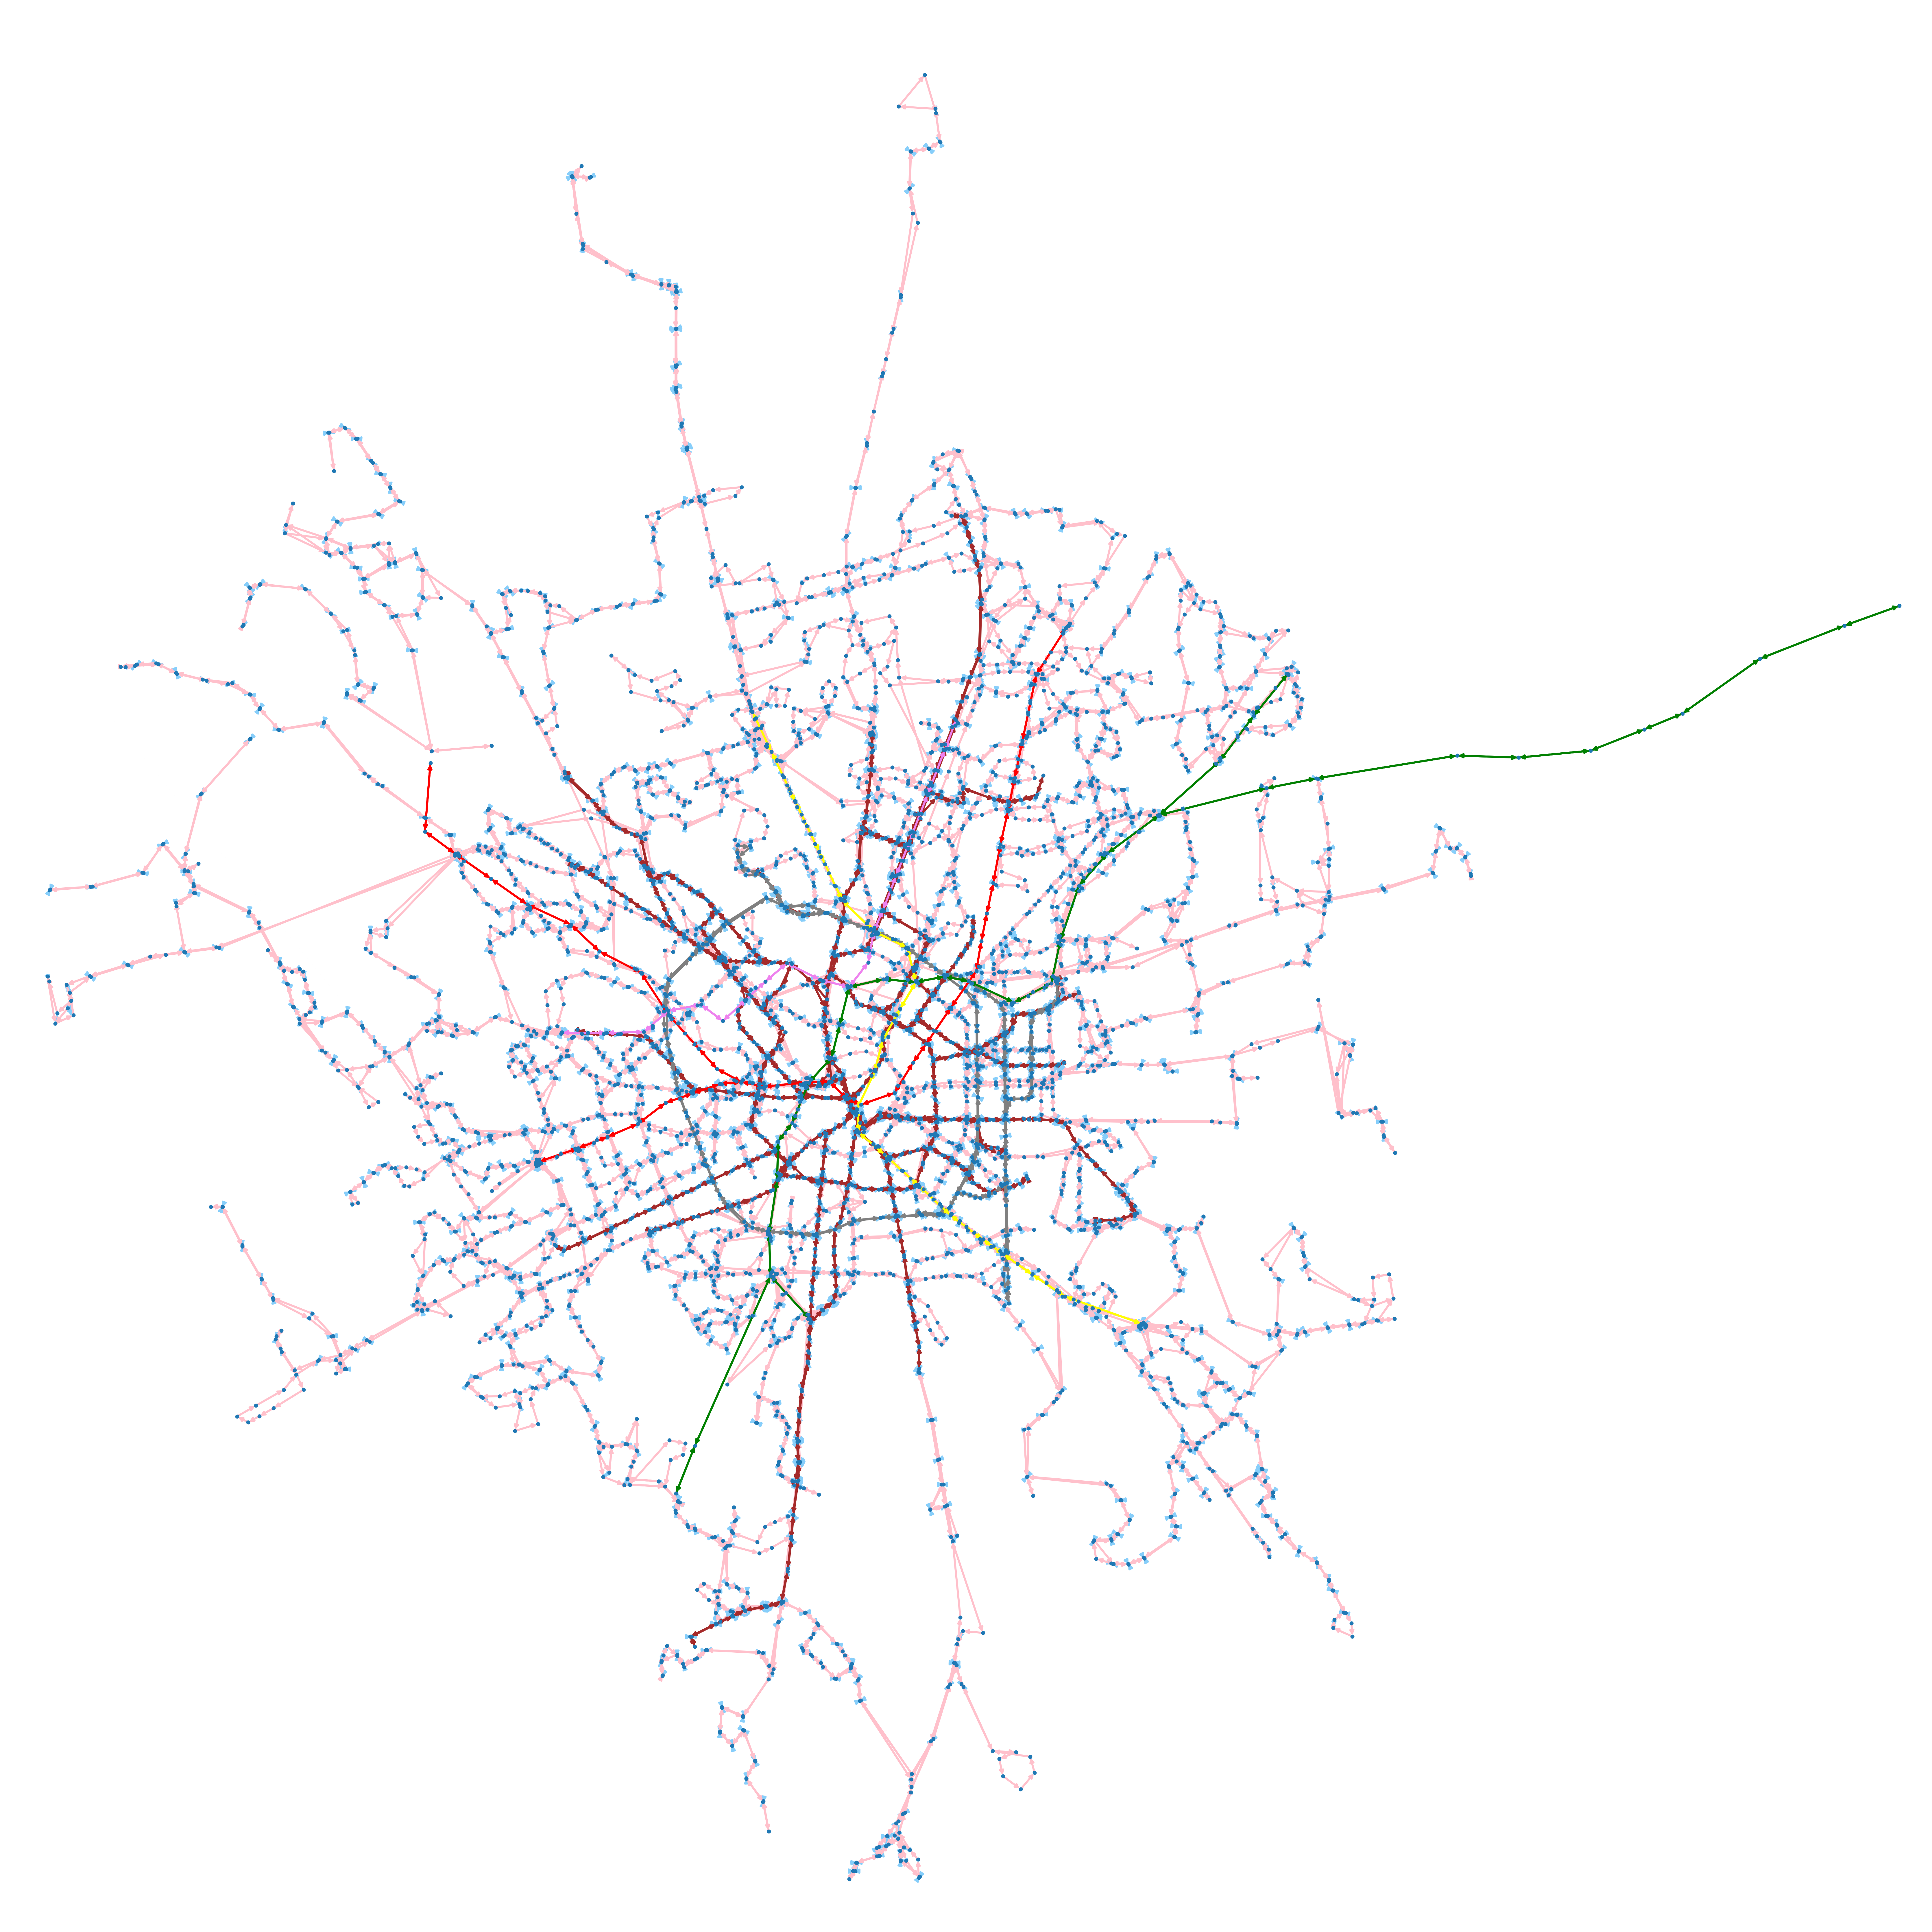
\includegraphics[scale = 0.5]{tex/pics/network_complete_cut.png}
    \caption{The public transportation network of Milan. Different transportation means are represented with different colors: metro line 1 is in red, metro line 2 in green, metro line 3 in yellow, metro line 5 in violet, tram in brown, bus in pink and filobus in gray. Walking paths, for ($r_{foot} = 200 m$), are shown in light skyblue.}
    \label{network_complete}
\end{figure}

%%%%%%%%%%%%%%%%%%%%%%%%%%%%%%%%%%%%%%%%%%%%%%%%%%%%%%%%%%%%%%%%%%%%%%%%%%%

 \section{The Agents}\label{sec:3.3}
 
Agents in the model represent the share of Milan's population which, during weekdays, moves around the city using public transports. I assume that the subpopulation of people moving regularly using public transports has the same distribution by age as the total population of residents, which can be found in \cite{site18}, updated to 2021. I only consider individuals that are older than 14 years old, and each agent belongs to one among 4 possible age classes: 15-24 years old ($\approx 11\%$ of the population), 25-44 years old ($\approx 30\%)$, 45-64 years old ($\approx 34\%)$ and over 65 years old ($\approx 25\%)$.
In this model we account for both systematic mobility, meaning the journeys made for study and working purposes, which happen regularly, and non-systematic mobility, namely those trips that take place less regularly and are attributable to reasons like meeting friends, eating out, going shopping or doing personal activities. I rely on Istat data about Italian population's use of time during an ordinary weekday \cite{site14}, updated to 2013. Agents start their daily routine at home, perform from 1 to 5 activities (among education, work, leisure, self-care/eating\footnote{Istat actually provides a category that includes eat, sleep and other self-care. However, given the time horizon I consider (5:00 a.m  to 1:00 a.m), I assume that “sleep” can be neglected.} and housework) and, eventually, go back home. \\
The creation of the synthetic population proceeds through different steps. First, for each agent I draw an age class from the distribution of inhabitants of Milan. Then, I draw a NIL for the agent's house from the distribution of the NILs conditional on the chosen age group \cite{site18}. Finally, I draw, uniformly at random from the stops in the selected NIL, a precise node which represents the agent’s home. 

At this point, two possible strategies can be adopted to assign a travel diary to the agents:
\begin{itemize}
    \item \textbf{Strategy 1.} For each of the five possible activities, I decide whether the agent will or will not perform it during the day, by drawing from a Bernoulli with parameter equal to the probability that the agent carries out such activity in an ordinary weekday, conditional on the agent's age class. Data used to construct this probability distribution come from data source 9. Adopting this strategy, each agent can have a variable number of activities to carry out, ranging from 1 to 5. The strategy is summarized in the algorithm \ref{alg1} below.
    \item \textbf{Strategy 2.} Agents are forced to perform a number $k$ of activities. The combination of activities to perform is drawn with replacement from the distribution of possible combinations conditional on the age group the agent belongs to. Specifically, I consider the choices of activities as independent of each other, so that the conditional probability of each combination corresponds to the product of the conditional probabilities of the single activities in it. The strategy is summarized in the algorithm \ref{alg2} below.
\end{itemize}

\pagebreak
\begin{algorithm}[H]
\caption{Agents' generation - strategy 1}\label{alg1}
\begin{algorithmic}
\Require $n \geq 0$
\For {each agent $i = 1, ..., n$}:
\State $\textit{age\_class} \sim Multinomial(p_l)$ \Comment{$p_l$ = P(age class l) for $l = 1, ..., 4$}
\State $\textit{nil} \sim Multinomial(q_{jl})$ \Comment{$q_j$ = P(nil j $\vert$ age\_class) for $j = 1, ..., 89$}
\State $\textit{home} \sim Uniform(k)$ \Comment{$ k = \frac{1}{\vert \{s: s \in nil \} \vert }$}
\For {each activity a = 1, ..., 5}:
\State $ \textit{u} \sim Bernoulli(f_a)$ \Comment{$f_a$ = P(a $\vert$ age\_class)}
\If{$u = 1$}:
    \State $\textit{destination} \sim Multinomial(g_s)$ \\\Comment{$ g_s = \frac{ \# \text{ amenities of type a close to node s}}{ \# \text{ total of amenities of type a}}$}
    \State $\textit{departure\_time} \sim Multinomial(r_t)$ \\\Comment{$r_t$ = P(travel time $\vert$ a) + U(-5, 5)}
\EndIf
\EndFor
\EndFor
\end{algorithmic}
\end{algorithm}

\begin{algorithm}[H]
\caption{Agents' generation - strategy 2}\label{alg2}
\begin{algorithmic}
\Require $n \geq 0$
\For {each agent $i = 1, ..., n$}:
\State $\textit{age\_class} \sim Multinomial(p_l)$ \Comment{$p_l$ = P(age class l) for $l = 1, ..., 4$}
\State $\textit{nil} \sim Multinomial(q_{jl})$ \Comment{$q_j$ = P(nil j $\vert$ age\_class) for $j = 1, ..., 89$}
\State $\textit{home} \sim Uniform(h)$ \Comment{$ h = \frac{1}{\vert \{s: s \in nil \} \vert }$}
\State \textit{activity\_combination} $\sim Multinomial(\theta_c)$
\\\Comment{$\theta_c$ = P(combination c $\vert$ age\_class) for $c = 1, ..., \binom{5+k-1}{k} $}
\For {each activity a = 1, ..., k in activity\_combination}:
\State $ \textit{u} \sim Bernoulli(f_a)$ \Comment{$f_a$ = P(a $\vert$ age\_class)}
\If{$u = 1$}:
    \State $\textit{destination} \sim Multinomial(g_s)$ \\\Comment{$ g_s = \frac{ \# \text{ amenities of type a close to node s}}{ \# \text{ total of amenities of type a}}$}
    \State $\textit{departure\_time} \sim Multinomial(r_t)$ \\\Comment{$r_t$ = P(travel time $\vert$ a) + U(-5, 5)}
\EndIf
\EndFor
\EndFor
\end{algorithmic}
\end{algorithm}
In the original version of the model, strategy 1 has been adopted. On average, using strategy 1, around $20\%$ of the initially generated agents come with no planned activities in their schedule and, therefore, are discarded. Experiments show that agents' schedules only contain 2 activities on average. To make the results of the two strategies comparable in terms of traffic load on the network, the parameter k for the second strategy will be set to 2 by default for following experiments. 

I assign a location to each activity selected for the agent (i.e. the specific node in the network) with probability proportional to the number of facilities corresponding to that task that are located nearby each node \cite{site9}. Among the possible categories proposed by OpenStreetMap, I only take into consideration the ones that match Istat activities (eg. schools, universities, etc. for education; offices, co-working place, etc. for work; cinema, gyms, etc. for leisure time; restaurants, bars, etc. for eat/sleep). When the activity “housework” is selected, I assign as destination of the trip the node corresponding to the agent’s house. I then appoint a departure time to each scheduled activity by drawing a 10-minutes time slot from the distribution of oriented movements over time, conditional on the specific activity \cite{site11} shifted back by 40 minutes, as I assume the activity will be performed approximately 40 min after the departure (40 minutes being the average traveling time according to \cite{bib2}). To allow for minute-by-minute departure times, I also include a randomization term that adds or removes at most 5 minutes from the picked time. 

Finally, if the last destination of the agent is not “home”, I compute a critical time at which the agent will depart again to go back home (time of the last activity + 40 min + average duration of last activity + noise in the [-10 min, +10 min] interval). I consider two possible sets of average duration for the activities:
\begin{itemize}
\item set 1: 120 min for sleep/eat/personal care, 330 min for education, 440 min for paid work and 90 min for free time;
\item set 2: 120 min for sleep/eat/personal care, 156 min for education, 220 min for paid work and 90 min for free time.
\end{itemize}
The numbers in the first set have been computed by averaging across age-classes the duration of activities from Istat data in \cite{site11}. In set 2 the average duration of education and paid work have been reduced by 50\%, as to allow for part-time occupations. 
The set used to compute the critical time is randomly chosen, for each agent, through a Bernoulli draw with parameter $p_{long}$ equal to the probability of choosing set 1 (the one with the longest average duration of activities). I set $p_{long}$ to 0.7 if the time of the last activities is before 1.30 a.m. and to 0.3 if it is after, as I believe that there is a higher chance of performing a long activity if that is started in the morning rather than in the second part of the day.
I assume that, if this critical time is after 10:30 p.m. the agent prefers not to use public transports to go back home, as the timetables are not favorable later in the evening. 


At this point, for each agent we have: a unique id, the age group, the starting point (node on the network) and a schedule of activities (from 1 to 5 activities, with the related destination and the time at which the agent has to start the journey to get there), as in the example in table \ref{tab1}. 


\begin{table}
\centering
\caption{Example of agent's generation}\label{tab1}
\begin{tabular}{ll|lll}
\multicolumn{2}{c|}{The agent} & \multicolumn{3}{c}{The schedule} \\ 
\toprule
Features      & Data      & Activity & Destination & Departure time \\ 
\midrule
Unique id & 7548 & 1) Education & V.le Bligny, 19 & 7:30\\
Age & 15-24  &  2) Work	& Duomo M3 & 14:15\\
Starting point & Corvetto M3 & 3) Leisure & Moscova & 19:25\\
\bottomrule
\end{tabular}
\end{table}

The final step to complete the synthesis of the population is to assign to each agent the list of edges that form the shortest path they will use to reach their destinations. Specifically, the shortest path is calculated through the Dijkstra algorithm, using as weight for each edge its traveling time. However, not all nodes are taken into account in this process. In fact, the shortest path is computed on the subgraph of the edges constituting the transportation lines that are active in a limited time window around the departure time. In this way, the agent can only select routes that are available at the time of their departure. This means that two agents who have been assigned the same couple of departure and destination stops may take two different paths to reach their common destination if the trips are scheduled at different times during the day. Lastly, since I am working on a multigraph, it may be the case that two stops are linked by two different means of transport with same speed. In this case, the agent includes in the shortest path the edges that minimize the number of changes of vehicles needed. 


Agents are characterized by a state, which can take four possible values: busy, waiting, traveling and finished. Busy agents are those that are currently in one of the facilities and do not have to travel. Waiting agents are the ones waiting at a stop in order to get on a vehicle. Traveling agents are situated on edges, and they are moving to their next destination. Finally, finished agents are those that have already completed all the journeys in their daily schedule. 

%%%%%%%%%%%%%%%%%%%%%%%%%%%%%%%%%%%%%%%%%%%%%%%%%%%%%%%%%%%

\subsection*{Validation of the synthetic population}\label{ssec:3.3.1}

Although the synthesis of the population is stochastic, as it involves multiple draws from different distributions of demographic and geographical features, choosing a large sample size allows to obtain samples of synthetic agents which resemble the true population. I estimate that the individuals take, on average, 8 different vehicles during the day: counting each time an agent takes a different vehicle as a separate passenger, if I start with 20000 agents then I get a total of 160000 synthetic passengers per simulation. If I treat each of them as representing 10 real people, and adjust vehicles' capacities accordingly, then I am able to run a simulation that represents the whole population of daily travelers on all the transport network of Milan, which amounts to 1590000 people, as reported in \cite{site20}. A sample size of 20000 agents is believed to be large enough to achieve low variability of agents' characteristics across different samples. To demonstrate this, I have generated 100 samples of 20000 synthetic agents, observed the distributions of multiple characteristics and computed means and standard deviations. The reported bar charts show that the observed distributions don't deviate significantly from the true ones. Numerical values for the means and standard deviations are available in the \nameref{appendix}.
One can easily see that the true relative proportions of age classes are preserved, with low standard error, as shown in figure \ref{pop_age}. Similarly, the estimated relative proportions of the population resident in each NIL resemble the true distribution, as shown in figure \ref{pop_nil_tot}. Details about the distribution of the population by NIL conditional on age classes are reported in the \nameref{appendix}. Another distribution observed is that of the combinations of activities performed by agents, under assignment strategies 1 and 2. The bar charts in figures \ref{pop_act} and \ref{pop_act2} show, on the left, in blue, the weighted average of the probabilities of the different combinations of activities, with weights equal to the proportions of the four age classes, and, on the right, in orange, the observed number of individuals per combination, averaged across samples. It is easy to see that variability across samples is low in both cases, and the observed proportions resemble the sampling distributions. Lastly, I compared the percentages of agents who have been scheduled to return home after their last activity across multiple runs, with 3 possible values for $p_{long}$, under the two different strategies. The averages for each combination are reported in figure \ref{p_long_as} and again the standard deviation is extremely low across runs.

\begin{figure}[H]
    \centering
    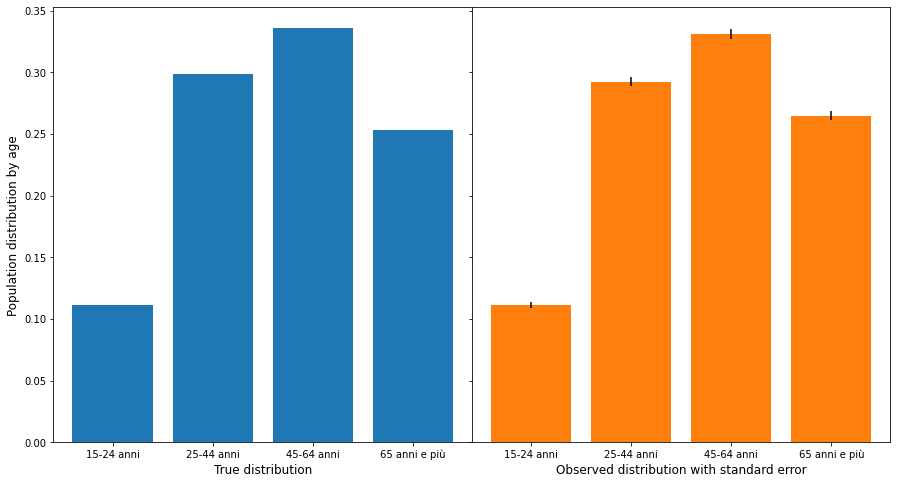
\includegraphics[scale = 0.5]{tex/pics/pop_by_age.png}
    \caption{Comparison between the true population distribution by age (in blue) and the observed one (in orange) with standard error, averaged across 100 samples.}
    \label{pop_age}
\end{figure}

\begin{figure}[H]
    \centering
    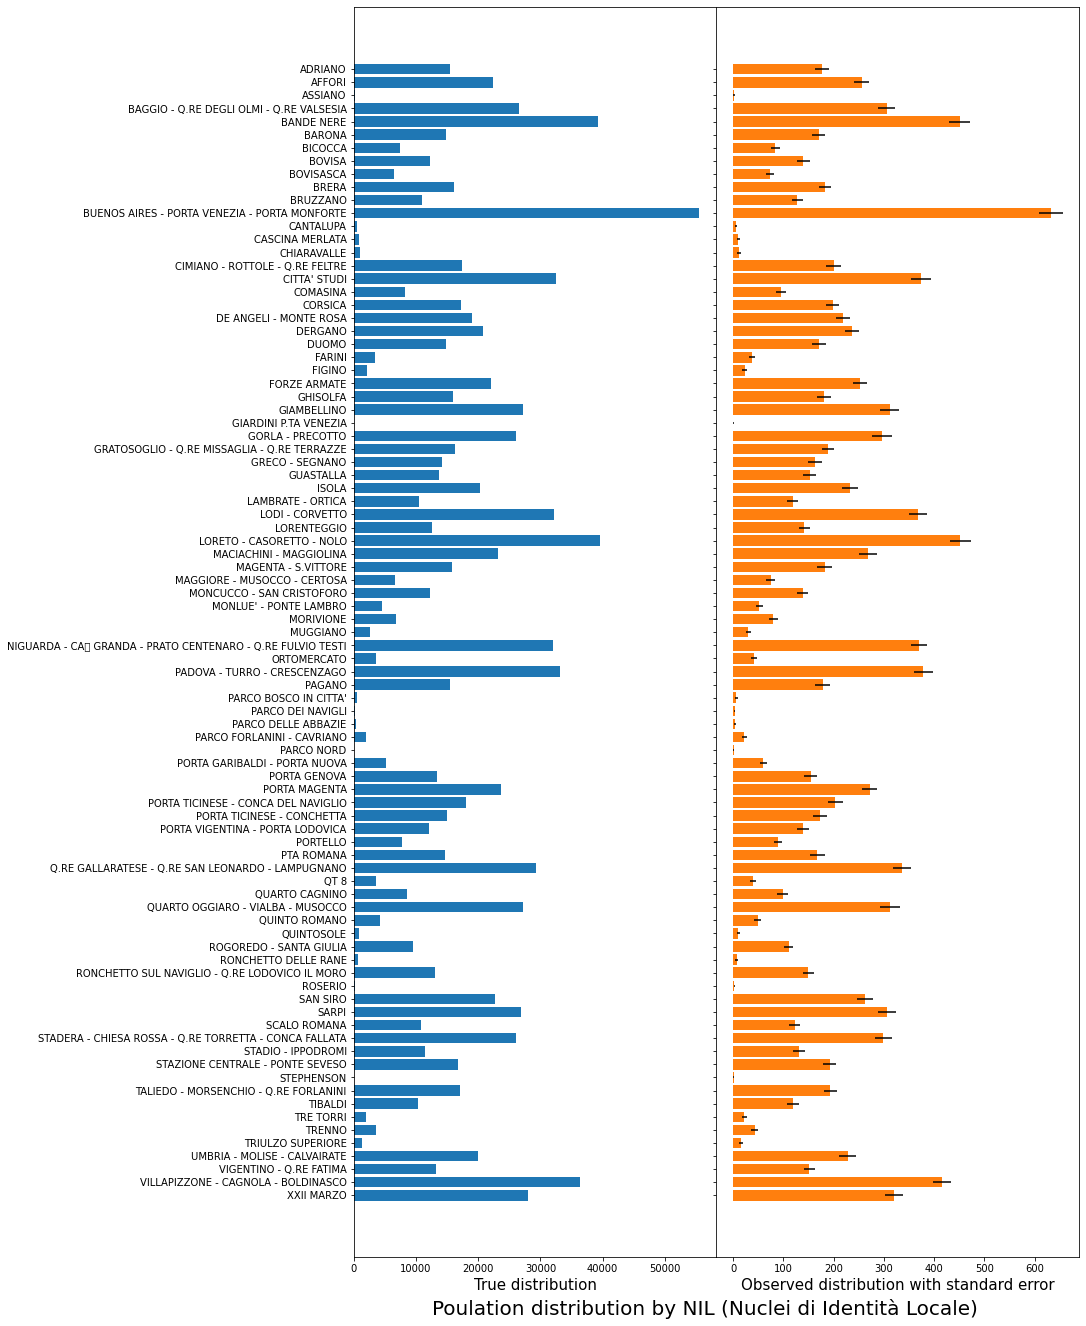
\includegraphics[scale = 0.45]{tex/pics/pop_by_nil_tot.png}
    \caption{Comparison between the true population distribution by NIL (in blue) and the observed one (in orange) with standard error, averaged across 100 samples.}
    \label{pop_nil_tot}
\end{figure}

\begin{figure}[H]
    \centering
    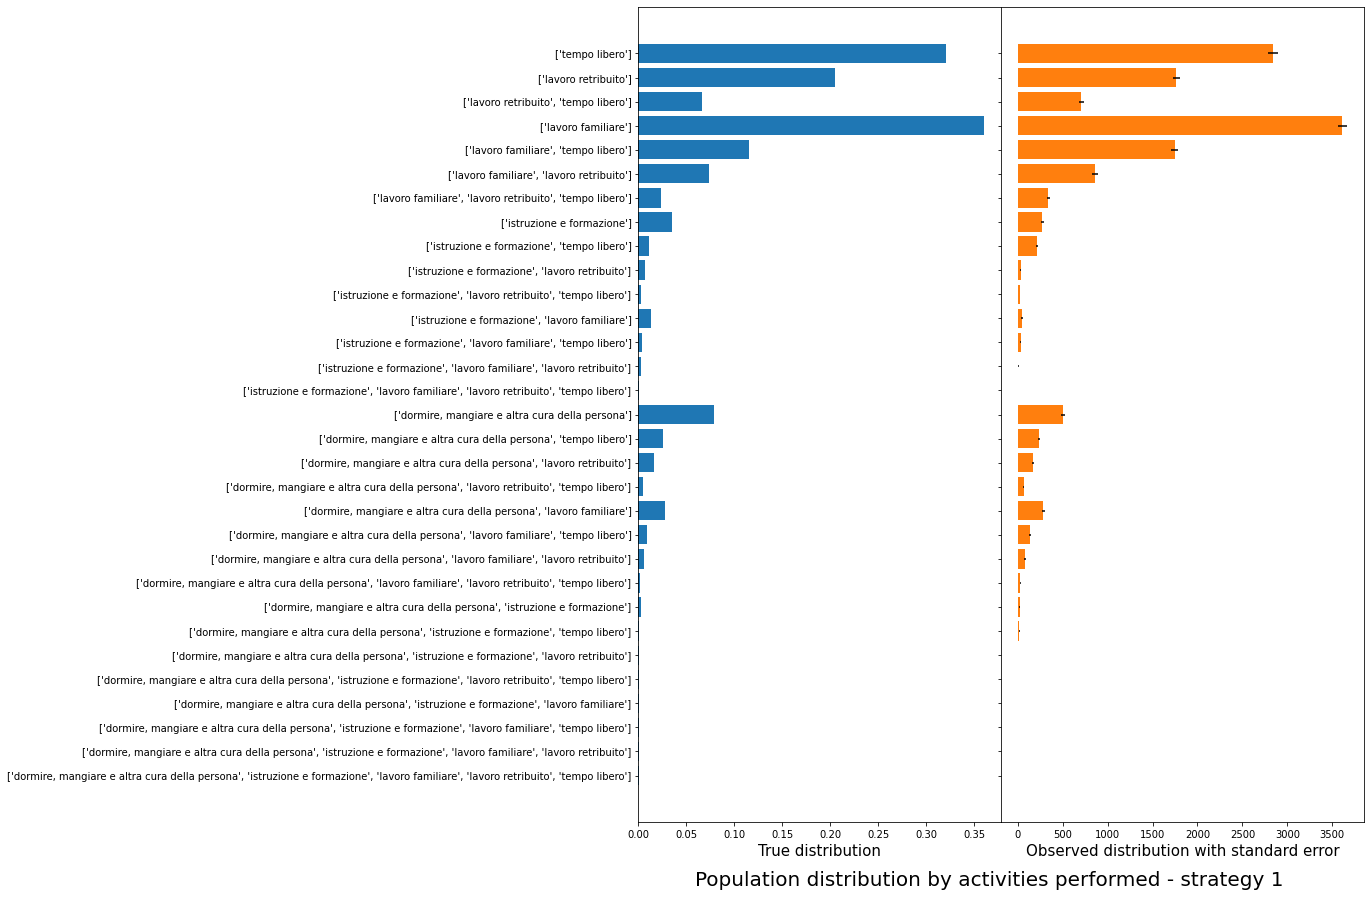
\includegraphics[scale = 0.35]{tex/pics/pop_by_act.png}
    \caption{Comparison between the true population distribution by activities performed (in blue) and the observed one (in orange) with standard error, averaged across 100 samples. Strategy 1 is used to assign activities to agents.}
    \label{pop_act}
\end{figure}

\begin{figure}[H]
    \centering
    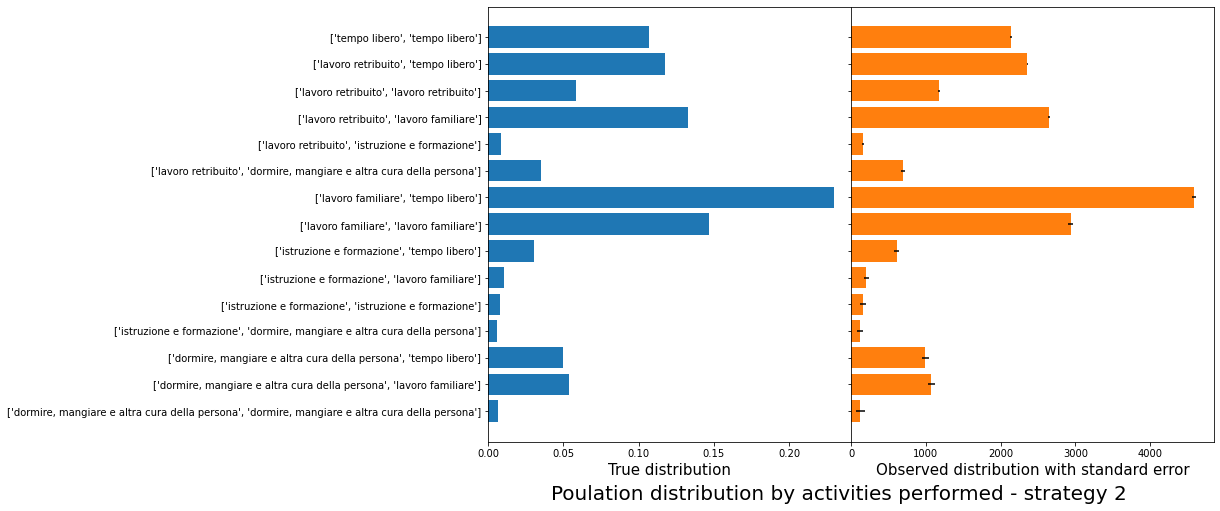
\includegraphics[scale = 0.4]{tex/pics/pop_by_act2.png}
    \caption{Comparison between the true population distribution by activities performed (in blue) and the observed one (in orange) with standard error, averaged across 100 samples. Strategy 2 is used to assign activities to agents.}
    \label{pop_act2}
\end{figure}

\begin{figure}[H]
    \centering
    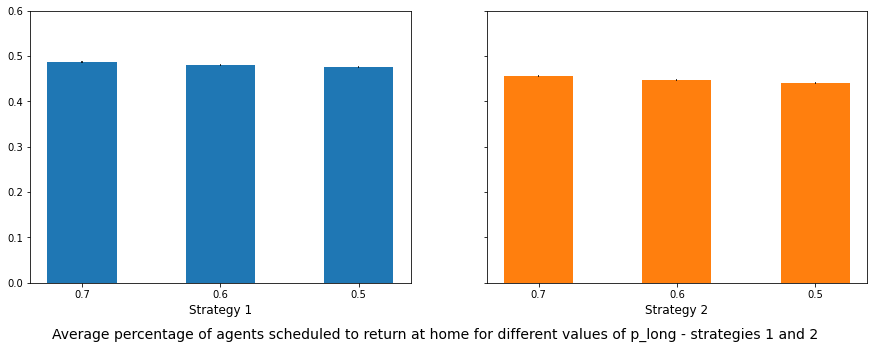
\includegraphics[scale = 0.4]{tex/pics/p_long_as.png}
    \caption{Comparison between the percentages of agents who have been scheduled to return home after their last activity across multiple runs, with 3 possible values for $p_{long}$, using the two different strategies.}
    \label{p_long_as}
\end{figure}

%%%%%%%%%%%%%%%%%%%%%%%%%%%%%%%%%%%%%%%%%%%%%%%%%%%%%%%%%%%%%%%%%%%%%%%%%%%
% \pagebreak
\section{The Rules}\label{sec:3.4}

Once the population of agents has been synthesized, all agents are initialized to the busy status and let move on the network to reach the destinations in their schedule. 
The typical simulation reproduces 20 hours, from 5:00 a.m. to 1:00 a.m. of the next day, but start and end time can be customized.
Each iteration of the simulation represents one minute. At each minute, I activate agents within groups in random order, to avoid giving the first-mover advantage to the same individual at each timestep. I first consider the set of “busy” agents: if they are scheduled to depart at the current minute, their status changes to “waiting”, otherwise, they remain “busy” at their current position. I then loop over the “traveling” agents: looking at their path, they evaluate whether they have to get off the current vehicle and disembark if that is the case. Clearly, they can only do so if the vehicle has gone across the edge and reached the next stop. Edges in the graph can be either active or inactive at any given time step: an edge is active at minute t if there’s a vehicle that is stopping at the starting node of the edge and can embark passengers. “Waiting” agents are the last to act: each of them looks at the next edge in their path and, if it is active and there’s space on the vehicle, they get on board, while, if that is not the case, they stay on the stop waiting for the next activation. Once an agent completes all of its tasks, its status changes to “finished” and it is no longer considered in the following iterations. It can happen that agents are scheduled to depart for an activity very late in the night, when rides are less frequent, so they fail to complete their journey, and their status never becomes “finished”. I assume that, in this case, they will use alternative ways, not covered in our model, to proceed. 

Now that we have described all the ingredients that characterized the model, we can summarize it by mapping its elements into the sets presented by Borgonovo et al. in \cite{Borgonovo2022SensitivityAO}:
\begin{itemize}
\item \textbf{Principles:} a principle of the model is that agents' houses are exactly on transport lines' stops. Indeed, the environment in this model is a network made of the points identifying stops and the lines connecting them, not the continuous Euclidean space representing the surface of Milan. This simplification seems reasonable, as I assume that the path from agents' houses to the closest stop is negligible. Hence, we can think of the departure times as the times at which an agent will be at the stop, ready to embark on a vehicle, rather than the times at which they plan to live their houses (or, more in general, their location). Another principle of the model is the characterization of agents through a state taking 4 possible values: busy, waiting, traveling and finished. A state determines the behavior of an agent in future steps. Making changes to the states system, for example as to allow for other admissible values for agents' state, would lead to a different model. 
\item \textbf{Assumptions:} an assumption of the model is that agents move on the environment representing the network of public transports of the city of Milan and have full knowledge of the network, so that they are able to plan in advance the path to follow in order to minimize traveling time. The current version of the network is built on data updated to 05/05/2022. Any update to the routes would result in a different version of the network, but that would not change the essence of the model. Similarly, one can adapt the model to a different city just by changing the network and timetables, if no modifications to the rules are made. I assume that agents are not aware of lines' timetables: they compute traveling time and base their choice of path on the assumption that the vehicles will be immediately available at the stop when they arrive.
\item \textbf{Parameters linked to the environment:} two important parameters of the environment are the capacity and speeds of vehicles, that determine the weights of edges and, hence, the expected traveling time agents consider when deciding which path to follow. Another important parameter is the maximum distance used to consider two stops as "at walking distance" ($r_{foot}$). This is crucial as it dictates the number of fictitious "foot" edges added to the original network and, consequently, the total number of possible paths available. Finally, one last parameter is $r_{pois}$, which I use to compute the number of points of interests that are reachable from each stop. This parameter plays an important role as it changes the probabilities of each activity being performed in proximity of any stop.
\item \textbf{Agents' Parameters:} the number of age classes and of possible activities the agents can perform are important parameters characterizing agents' profiles. The distributions of the age classes and of NILs given age class are multinomial distributions whose parameters need to be mentioned among agents' parameters. Moreover, the probability of agents performing "long" tasks rather than short ones, $p_{long}$, is an important parameter which influences agents' decision to return back home with public transports at the end of their schedule.
\item \textbf{Procedures:} some procedures describe the way in which agents are able to embark vehicles: first traveling agents get off, then waiting agents try to get on in random order, succeeding unless full capacity of the vehicle is reached. Another relevant procedure is the strategy used to sample activities: the standard one is to allow for one possible occurrence of each activity during the day, while, an alternative is to allow for repetitions of each activity up to a number k of total activities. 
\end{itemize}

%%%%%%%%%%%%%%%%%%%%%%%%%%%%%%%%%%%%%%%%%%%%%%%%%%%%%%%%%%%%%%

\section{Simulation outputs and experiments}\label{sec:3.5}
During the simulation, the researcher is able to collect measures and statistics about the agents, which help evaluate the state of the system and the effects, in terms of flow and overload, of shocks and interventions. 
In particular, interesting KPIs are:
\begin{itemize}
    \item total waiting and traveling time;
    \item total waiting and traveling time per trip;
    \item percentage of traveling and waiting agents at each time step;
    \item total number of vehicle changes;
    \item total number of minutes each edge reaches its full capacity;
    \item total number of times an agent travels on foot;
    \item total number of passengers on each vehicle during the day;
    \item total number of agents passing on each node and each edge;
    \item maximum number of simultaneous agents on an edge (maximum load reached by the vehicle);
    \item distance-adjusted time-per-trip distribution, meaning the distribution of agents by the time it takes for them to cover 1 km.
\end{itemize}

The proposed model allows to test the effects of the implementation of measures already enforced in reality, and to make forecasts about possible scenarios that have not been realized yet, provided that data about the network structure and transport timetables after the changes are available.
Experiments have been conducted to evaluate two realistic scenarios:
\begin{itemize}
    \item \textbf{Suspension of metro stop "Duomo"}, both in metro line 1 and metro line 3. This intervention is usually implemented in Milan when big events, such as concerts or shows, are organized in Piazza Duomo, in order to preserve public security and reduce the affluence to that stop that could be overcrowded: ATM temporarily interrupts the possibility to get out of the Metro 1 and Metro 3 in Duomo, allowing direct connections between the immediately previous and subsequent stops of the metro line.  
    \item \textbf{Introduction of the new metro line 4}, which is expected by the end of 2023. The route comprehends 21 stops, and it aims to connect the western side of Milan, from San Cristoforo, to Linate Airport.
\end{itemize}
In order to account for the uncertainty due to the population synthesis' stochasticity, 10 separate simulations per each phase of each experiment have been run and results have been aggregated. For each experiment, 10 groups of, on average, 20,000 agents have been initialized\footnote{Activity assignment has been conducted adopting strategy 1, which, on average, discards 20\% of agents, having empty schedule. Therefore, to obtain a net sample size of approximately 20000, the number of agents to generate has been set to 25000.}, each one representing 10 real passengers. \\
The experiments consist of two phases, one before and the other after the network changes, in which the same samples of agents are used. The impact of the interventions is evaluated comparing the average waiting time and traveling time before and after the intervention, both for the set of involved agents (those whose paths were affected by the shock) and the whole sample of agents. Moreover, I am able to isolate the most and less impacted lines and also the route sections experiencing the highest load during the day.